\chapter{Zahtjevi aplikacije i korištene tehnologije}
U ovome poglavlju opisani su zahtjevi koje aplikacija mora zadovoljiti i tehnologije koje su bile korištene u njenoj izradi. 

\section{Zahtjevi}

Zahtjevi su 
podijeljeni na:
\begin{enumerate}
    \item Korisničke
    \item Funkcionalne
\end{enumerate}

Korisnički zahtjevi predstavljaju zahtjeve samoga korisnika, tj. što aplikacija mora omogućiti korisniku.
Funkcionalni zahtjevi služe identifikaciji glavnih funkcija sustava i omogućuju kvalitetniju izradu same
aplikacije.

\subsection{Korisnički zahtjevi}
\subsubsection{Omogućen odabir načina detektiranja objekata} 
Unutar aplikacije moguće je odabrati između statičkog i dinamičkog detektiranja
objekata. Pojam dinamičkog detektiranja odnosi se na detekciju u stvarnom vremenu. Statičko detektiranje mora moći podržavati odabir fotografije iz galerije, ali i snimanje nove fotografije nad kojom se 
izvodi detektiranje. Za detekciju u stvarnom vremenu otvara se kamera čime počinje postupak detektiranja. 

\subsubsection{Prikaz rezultata na zaslonu}
Aplikacija mora moći prikazati podatke dobivene iz ulazne slike ili videozapisa korisniku. Rezultat mora biti prikazan 
kao okvir oko detektiranog objekta, te ime razreda kojem objekt pripada.

\section{Funckionalni zahtjevi}
\subsubsection{Učitavanje sadržaja}
Aplikacija mora podržavati učitavanje sadržaja iz različitih izvora. Prilikom učitavanja fotografija iz galerije 
ne postoje dodatni zahtjevi, dok se kod korištenja kamere mora prvo provjeriti postoji li na uređaju kamera.
\subsubsection{Učitavanje modela}
Model mora biti učitan lokalno. Aplikacija se ne smije spajati s udaljenim poslužiteljem kako bi se izbjegla ovisnost o internetskoj vezi. 

\section{Tehnologije}
Za implementaciju modela detekcije objekata korištene su različite tehnologije bez kojih bi postupak bio značajno otežan i 
skloniji pogreškama.
\subsection{Tensorflow}
Tensorflow je Googleova biblioteka otvorenog koda. Služi kao sučelje za uporabu algoritama strojnog i dubokog učenja, te implementaciju
istih. Korisnik se koncentrira na izgled modela i slojeve koji su zastupljeni u samom
modelu, dok će Tensorflow brinuti za ostale postupke koji se događaju u pozadini. Širok je spektar proizvoda koji se mogu razvijati pomoću
Tensorflowa, kao što su: 
\begin{itemize}
    \item Segmentacija 
    \item Klasifikacija
    \item Detektiranje poze
\end{itemize}
Fleksibilna arhitektura Tensorflowa omogućuje korisniku razvoj i pokretanje modela
na procesoru, grafičkoj kartici, pa čak i TPU \engl{Tensor processing unit}.
Mobilna inačica Tensorflowa naziva se Tensorflow Lite. 
Razlog razvoja ove inačice bila je sve veća količina podataka koju su mobilni uređaji 
mogli pohraniti, ali i sve veća procesorska snaga. Milijuni korisnika diljem svijeta u svakom 
trenutku koriste svoje mobilne uređaje za neke određene zadatke, te nije praktično imati model na 
udaljenom poslužitelju kojemu se pristupa putem mobilnog uređaja. Tensorflow Lite značajan je za daljnji razvoj i 
implementaciju modela dubokog i strojnog učenja, jer eliminira potrebu za spajanjem na poslužitelj i ubrzava postupak dobivanja
rezultata od modela.\citep{tensorflow2015-whitepaper}

% \begin{figure}[htb]
%     \centering
%     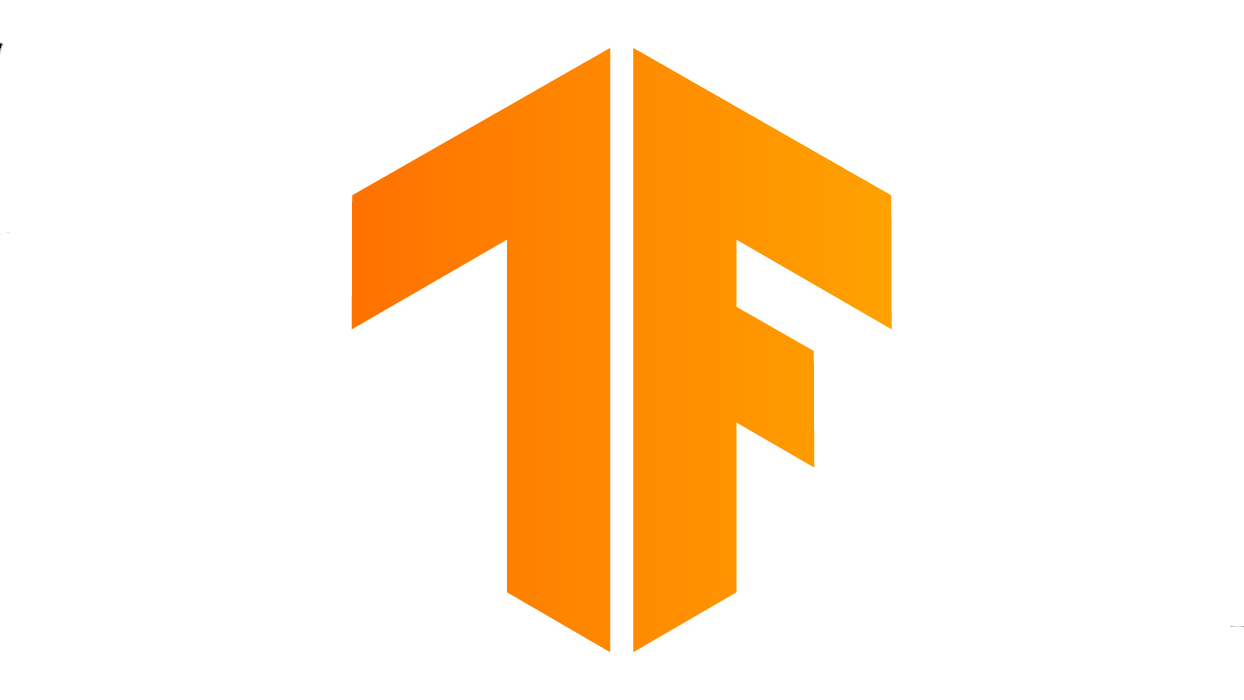
\includegraphics[width=10cm]{img/tensorflow.png}
%     \caption{Tensorflow je jedna od najpoznatijih biblioteka otvorenog koda. Slika je preuzeta s https://www.tensorflow.org/}
%     \label{Tensorflow}
% \end{figure}


\subsection{Flutter}
Razvoj mobilnih aplikacija u današnje je doba od velike važnosti zbog sve veće globalne potražnje. Dvije mobilne platforme koje imaju najveći udio na 
tržištu su Appleov IOS i Googleov Android. Vještine u izradi aplikacija i sustava za ove platforme izrazito su tražene. Problem je međutim naći programere koji
istodobno rade na obje platforme, budući da se za razvoj aplikacija koriste različiti jezici i radni okviri. 
Radni okvir Flutter nastoji riješiti ovu poteškoću tako što nudi mogućnost prevođenja koda za IOS i Android, ali sve iz iste baze koda. 
Nastao je u Googleu 2017. godine, kada je mogao jedino prevoditi kod za Android operativni sustav. Programski jezik koji se koristi za razvoj unutar ovog okvira naziva se Dart. Ovaj jezik također je razvijen u Googleu. 
Glavna komponenta u Flutteru su "Widgeti". Služe za prikaz elemenata na ekranu. Dva skupa ovih komponenti koje postoje unutar radnog 
okvira su Material Design (Android) i Cupertino (IOS).
U najnovijoj inačici Fluttera postoji mogućnost pokretanja aplikacija kao web aplikacije. Ova mogućnost još uvijek je u beta razvoju. 

% \begin{figure}[htb]
%     \centering
%     
\includegraphics[width=10cm]{img/flutter.png}
%     \caption{Flutter omogućuje razvoj aplikacija za više platformi. Slika je preuzeta s https://flutter.dev}
%     \label{Flutter}
% \end{figure}


